\section{Graf momentov $M(p_T)$}
Naslednja naloga je bila izrisanje grafov momentov posameznih jetov razporejenih
na intervalih transverzalnih gibalnih količin jetov. Znotraj vsakega jeta je bil izračunan moment,
in je bil podeljen intervalu. 
Moment jeta je bil izračunan po formuli:
\begin{equation}
    M_{i_J} = \sum_{k}^{N_J}R_k^i \frac{p_{T_k}}{p_{T_J}}
\end{equation}
Indeks $i$ predstavlja tip momenta.
Znotraj vsakega intervala sem izračunal povprečen moment in ga 
grafično upodobil z modro piko, kot je prikazano na sliki: 
\begin{figure}[h]
    \begin{center}
        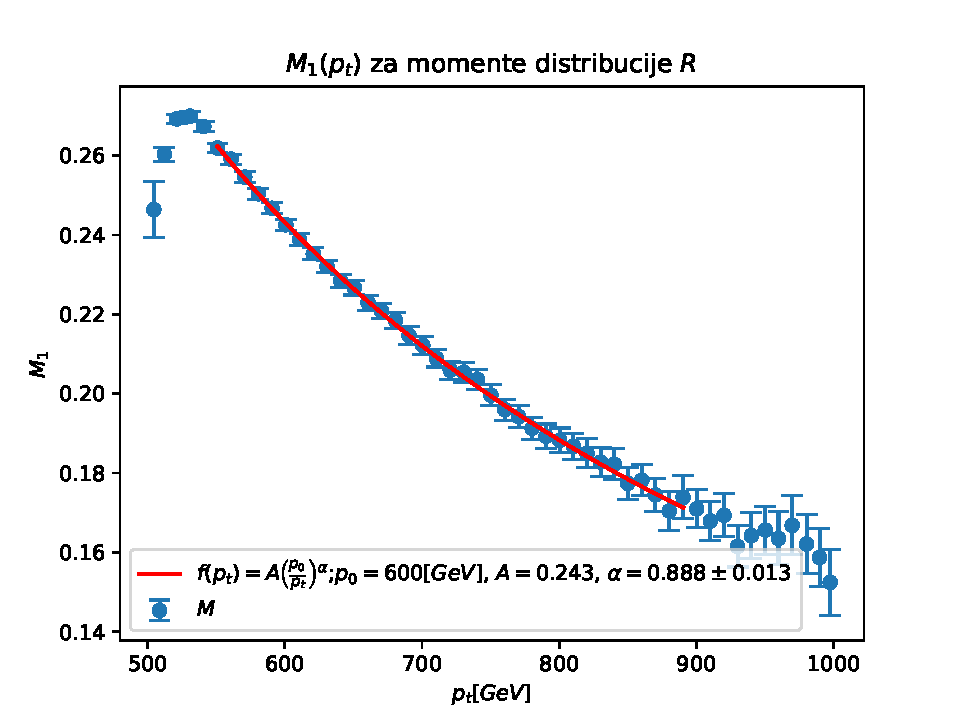
\includegraphics[width=13cm]{sections/section3/figures/CCM_1(P_t).pdf}
        \caption{Graf $M(p_T)$ za momente distribucije $R$, s fitano funkcijo oblike $f(p_T) = A\left(\frac{p_0}{p_T}\right)^\alpha$ od $550$ do $900$ GeV/c}
        \label{slika 4}
    \end{center}
\end{figure}
\\
Grafu sem dorisal absolutno napako, ki je bila izračunana s pomočjo standardne
devijacije. 
\begin{equation}
    \Delta M_{j} = \sqrt{\frac{\sum_{k}^{N_j} \left(M_{jk} - \overline{M_j}\right)^2}{N_j^2}}\;\cdot\; 1.96
\end{equation}
Indeks $j$ označuje zaporedni interval (bin), indeks $k$ pa označuje posamezen moment v intervalu $j$,
$\overline{M_j}$ je povprečna vrednost $M$ znotraj intervala $j$, ter $N_j$
označuje število momentov na intervalu. Število $1.96$ nastopa v enačbi zato,
da napaka zajame $95\%$ podatkov.
Fit funckcije je bil narejen s pomočjo \verb|scipy.optimize.curve_fit()|.
\\
\\
Slike so shranjene v datotekah 
\verb|CCM_i(P_t).pdf|, kjer je $i$ spet število momenta. Sama koda, ki zgenerira tako sliko, je shranjena v
\verb|CCM(pT).py|
\subsection{Graf momentov $M(p_T)$ za distribucije $R^2$}
Podobno kot smo v pogavlju \ref{section2} najprej narisali graf 
za $R$ in potem $R^2$ lahko sedaj naredimo isto. Za $R^2$ vemo formulo iz enačbe \eqref{5}.
\begin{figure}[h]
    \begin{center}
        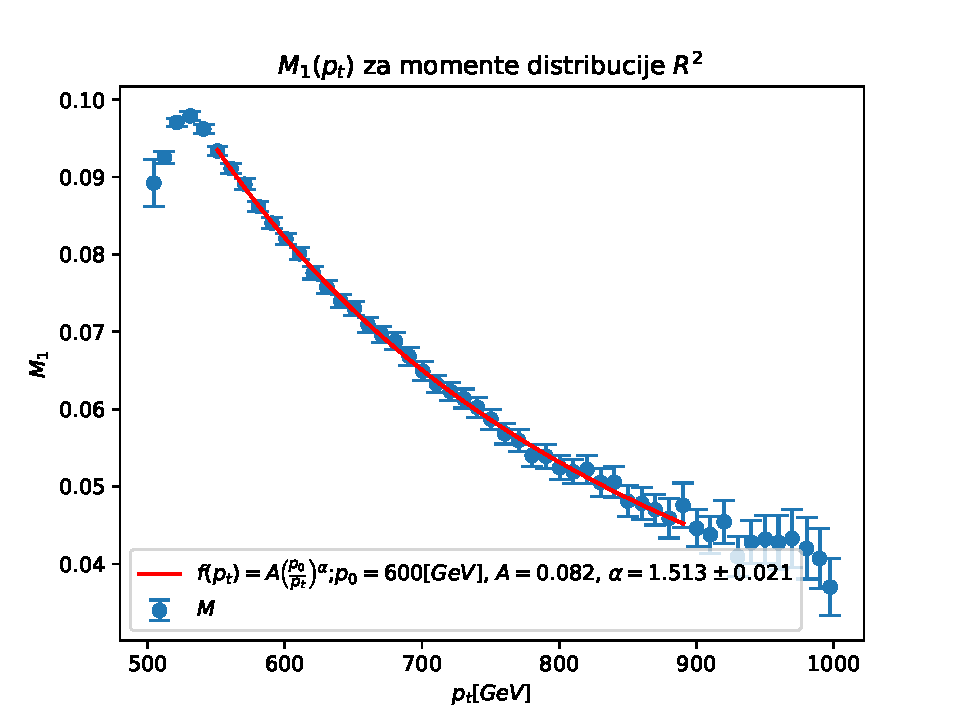
\includegraphics[width=13cm]{sections/section3/figures/M_1(P_t).pdf}
        \caption{Graf $M(p_T)$ za momente distribucije $R^2$, s fitano funkcijo oblike $f(p_T) = A\left(\frac{p_0}{p_T}\right)^\alpha$ od $550$ do $900$ GeV/c}
        \label{slika 5}
    \end{center}
\end{figure}
\\
Grafi za momente distribucije $R^2$ so shranjeni pod imenom \verb|M_i(P_t).pdf|, koda pa v
\verb|M(Pt).py|